\documentclass[aasms,12pt]{article}
\usepackage{natbib}
\setlength{\bibsep}{0pt plus 0.3ex}
\usepackage{sectsty}
\usepackage{graphicx}
\usepackage{epstopdf}
\usepackage[skip=2pt,font=small]{caption}
\captionsetup{width=\textwidth}


%\usepackage{titlesec}
%
%\titlespacing\section{0pt}{12pt plus 4pt minus 2pt}{5pt plus 2pt minus 2pt}
%\titlespacing\subsection{0pt}{12pt plus 4pt minus 2pt}{0pt plus 2pt minus 2pt}
%\titlespacing\subsubsection{0pt}{12pt plus 4pt minus 2pt}{0pt plus 2pt minus 2pt}


\sectionfont{\normalsize}
\usepackage{fullpage}

%\usepackage[margin=1in]{geometry}

%\citestyle{aa}
\newcommand{\sol}{\ensuremath{\odot}}


\usepackage{fancyhdr}
\pagestyle{fancy}
\fancyhf{} % sets both header and footer to nothing
\renewcommand{\headrulewidth}{0pt}
\cfoot{\thepage}
\rfoot{\footnotesize{Evan Anders, NASA NESSF 2015}}




\begin{document}
\begin{center}
   \large\textbf{The solar dynamo: Understanding the tachocline's role and bridging
	the gap between simulation and observation}\\
   \vspace{0.4cm}
   \large{Evan Anders}\\
   \vspace{0.4cm}
   \normalsize\textit{Advisor: Benjamin Brown}\\
   \normalsize\textit{LASP, University of Colorado at Boulder}\\
\end{center}



\abstract{Dynamo action
	powered by solar convection causes the Sun to be magnetically
	active.  The workings of the solar magnetic dynamo have been greatly
	informed by numerical simulations.  
	Traditionally, these simulations
	have described solar-type stars with high rotation rates
	and large characteristic convective motions compared to solar values.
	Here I propose a
	suite of 3-D numerical simulations of the solar convective zone
	with accurate solar rotation and convective velocity profiles, developed
	using the state-of-the-art anelastic spherical harmonics (ASH) code.  
	My primary
	goal is to determine the role of the solar tachocline, the rotational
	shear layer at the base of the convective zone, in the production
	and sustenance of the solar magnetic dynamo.  Furthermore, I propose
	a set of simulations of increased complexity that will include the 
	supergranulation of the solar photosphere for the purpose of
	post-processing to create
	synthetic observables.  Such mock-observables will be 
	compared directly to data gathered by the Solar Dynamics 
	Observatory and used to predict observations of the upcoming Solar 
	Orbiter.  This project supports objective 1.4 of NASA's 2014 Strategic Plan
	and will assist in developing ``the
	knowledge and capability to detect and predict extreme conditions in
	space'' in accordance with NASA's overarching Heliphysics science goals.}



\section{Introduction}
The Sun is a magneticly active star.  Its magnetism arises from an 
organized dynamo seated in the turbulent plasma
motions of the solar convective zone, which occupies roughly the outer 30\%
of the Sun's radius.  In the presence of
convective motions, magnetic fields and solar rotation couple to produce global
wreaths of magnetism which drive the Sun's 22-year cycle of magnetic activity.
This activity manifests itself in the collection of phenomena generally
referred to as solar activity, including magnetic storms and coronal mass
ejections.  Such activity propagates towards Earth, threatening disruption of 
power
grids and aircraft operations and endangering astronauts and satellites.  It is
clear that the Sun's magnetism affects our increasingly technological society;
understanding the nature of the dynamo that drives solar magnetism is of
paramount importance (\citealt{Toomre2009, Charbonneau2014}).

While current simulations lack the power to predict accurately 
the stellar magnetic environment 
over long time scales, they have provided great insight into the mechanisms
underlying the solar dynamo over the past decade.  
It is observationally proven that the surface of the sun rotates differentially,
and that the poles rotate roughly every 35 days while the equator rotates every 25
days.  By probing the Sun's
radial structure and sub-surface convective flows using acoustic oscillations,
helioseismology
has revealed that the solar differential rotation profile extends through the
bulk of the convective zone and has two distinct shear regions.  A near-surface
shear layer occupies roughly the outer 5\% of the Sun. A secondary shear
layer, called the tachocline, 
separates the differentially rotating convective zone from the uniformly
rotating radiative zone located radially inward.  
Traditional models of the solar dynamo, namely Babcock-Leighton flux-transport
dynamo models and interface dynamo models, state that the
tachocline drives the production of toroidal magnetic   
fields that fuel the solar dynamo and manifest at the solar surface as
sunspots and active regions.  In such models, magnetic fields generated
in the convective zone are transported inward to the tachocline, where
magnetic wreaths are built before buoyantly 
rising to the solar surface (\citealt{Toomre2009}).

Meaningfully creating numeric simulations of the 
solar environment requires working with wide ranges
of spatial and temporal timescales.  However, the
underlying equations at the heart of these magnetohydrodynamic (MHD) 
simulations---which express conservation of mass, momentum, and energy and
account for magnetic induction---are simple (\citealt{Charbonneau2014}).  Most current
simulations
have studied stars with higher rotation rates than the Sun, as the strength
of the magnetic dynamo increases proportionally to the stellar
rotation rate (see Fig.
\ref{wreaths}\emph{a}).  Such simulations
have informed solar dynamo theory and generated 
self-sustaining, buoyantly-rising toroidal wreaths of magnetism with polarity
shifts on long time scales,
shown in Fig. \ref{wreaths}\emph{b\&c}.  

\begin{figure}[t!]
\centering
\includegraphics[width=14cm]{figs/Pizzolato_and_D5.eps}
\caption{(a) Observationally measured stellar
        x-ray luminosity is plotted versus stellar rotation period.  There is a 
	clear increase in x-ray luminosity (powered by stellar magnetism) 
	as rotation
        period decreases (\citealt{Pizzolato2003}).  (b) Global scale toroidal 
	wreaths of magnetism have been obtained using the ASH code to numerically
	simulate Sun-like stars.  There is a clear polarity inversion in which the
	simulation fields cyclically reverse (c) every five years
        (\citealt{Brown2011}).
        \label{wreaths}}
\end{figure}


In light accepted dynamo theory, an unsettling result has arisen
in recent simulations of Sun-like stars.  Recent simulations disagree
on whether the tachocline is a necessary ingredient
in the sustenance of the solar magnetic dynamo.  Cyclic, Sun-like dynamos
have been
achieved in 3-D numerical simulations both with
(\citealt{Ghizaru2010, Racine2011})
and without (\citealt{Brown2011, Nelson2013}) the presence of a tachocline. This
begs the fundamental question: does the solar toroidal magnetic field---and, thus,
the solar dynamo---require the presence of a tachocline?
Those simulations which produced opposing
results were created using different codes and differing models for subgrid
processes at various stellar rotation rates.  Consequently, it is impossible to
compare the results of the simulations directly.  The data required
to determine the role of the tachocline are missing.

Additionally, most simulations
of solar convection simulate Sun-\emph{like} stars rather than the Sun
itself.  Such simulations model stars with greater rotation rates and 
convective flow velocities than the Sun.  Furthermore, it has recently 
been discovered
that these simulations self-consistently achieve amplitudes of 
large scale convective motions much larger than those present in 
the Sun
(\citealt{lord2014}).  Such a discrepancy calls for a new set of solar 
numerical simulations which more accurately describes convective flows.
The Rossby number, the ratio of convective timescales to rotation timescales,
appears to control the nature of global-scale dynamo action.  At low Rossby
numbers, cycles and global organization emerge self-consistently.  By lowering
the convective amplitudes, we can achieve the low Rossby regime at solar
parameters.  This allows us to explore the physics of the global-dynamo action
in the Sun itself, rather than making inferences about the solar dynamo from
rapidly rotating solar-like stars.

While simulations of stellar magnetic dynamos have proven
irreplaceable in gaining insight into the structure and evolution of 
long-term cycles, they fail to realate to \emph{in-situ} measurements
of solar magnetism and cannot provide insight on short time scales.
With the wealth of spacecraft either currently or soon-to-be 
gathering data on the Sun, now is the time to bridge the gap between 
theoretical dynamo simulations and direct observations of solar activity.


\section{Does the tachocline drive the Sun's toroidal magnetic fields?}
I propose a set of MHD simulations of the Sun's convective zone
to test the tachocline's role in generating the solar magnetic 
dynamo.  These simulations will model the solar convective
zone from its base up to the base of the outer convective shear layer, stopping
around $R = 0.97R_{\odot}$.  These simulations will include identical rotation
rates and convective timescales, but one simulation will include the shear
effects of the tachocline by extending down to about 0.5 $R_{\odot}$
while the other simulation will stop at the base of the convective zone
around 0.713 $R_{\odot}$, neglecting the tachocline.  
The background stellar structure (taken from a MESA solar model) will be 
otherwise identical between the simulations.
Dynamo theory champions the tachocline as the seat of the toroidal component
of the solar magnetic field, and it is time to put this theory to the test.
By building two simulations which are identical other than the presence or lack
of a tachocline, we can directly test this theory.  The data from such
simulations can provide greater certainty regarding the importance
of the tachocline in the generation and maintenance of the solar dynamo.

I will use the Anelastic Spherical Harmonic (ASH, 
\citealt{Clune1999}) spectral solver, which I will have access to through my
advisor, Dr. Benjamin P. Brown, to create my simulations.  The ASH code is the
current state-of-the-art code for modeling the global solar dynamo
(\citealt{Toomre2009, Brun2011, Alvan2014}). The use of a such a 
well-established code will allow me to
efficiently simulate the solar convective zone in spherical coordinates and gain
and understanding of the physics at work without having to
worry about generating a fully functional solving suite.  
Naturally, work
of this magnitude requires access to massively parallel computing resources.
As a CU Boulder student, I have access to the school's local supercomputer,
\emph{Janus}.  Additionally, I will work with Ben Brown to acquire CPU time on
state-of-the art supercomputers such as the NSF XSEDE resources and NASA's
\emph{Pleiades}. 

I have been well prepared by my past education to undertake
simulations of this magnitude.  
In 2012, I worked with
Pacific Northwest National Laboratory's (PNNL) Data Intensive Scientific
Computing group and gained an understanding of the challenges that are
faced in the
creation of large, scientific computations.  In addition to learning the
struggles faced in efficiently creating massively parallelised algorithms,
I learned how to effectively understand and utilize computational tools
(such as ASH). I also learned
techniques for debugging and optimizing my routines.

Additionally, over the summer of 2013 I participated in the NSF Science
Undergraduate Research Fellowship program at the Laser Interferometer
Gravitational-wave Observatory (LIGO).  During my time at LIGO Hanford, it was
my task to create a computational tool which analyzed LIGO science run data at
specific frequencies and output those analyses
in user-friendly text files.  This experience taught me how to interact with
massive quantities of data, how to organize that data meaningfully in files,
and how to effectively plot and visualize such data.  All of these skills
will be exceptionally useful at all stages in the creation of 
massive 3-D simulations.

In addition to my strong undergraduate education in physics, I am in the process
of learning the fundamentals of fluid mechanics and plasma physics necessary to
understand and implement the MHD processes governing motion within the solar 
convective zone.

\section{Simulated observables: Connecting observations and simulations}
While simulations provide great insight into the
physical trends occuring within a system, they often fall short of a direct
connection to observable data.  Thus, I propose a second suite of simulations
that spans the entirety of the solar convective zone and reaches out to
the solar photosphere to display the behavior of magnetic fields
at the observable surface of the Sun.  In efforts to accurately portray the
physics at work, these simulations will capture supergranular 
scales.  
Including supergranular scales at the photosphere will allow us to explore the
emergence of active regions and their coupling to deep magnetism.
Small scale granulation will be ignored for two reasons.  
First, the motions of granulation are roughly two orders of magnitude
smaller than the motions of the vast solar convective zone, making granular
contributions unimportant.
Second, the computational load of resolving granular scales
would push our simulation workload past a feasibly acquirable number of CPU
hours on state-of-the-art machiens.

Numerous post-processing techniques will be used on the photospheric data 
produced by these simulations in order to create synthetic observables.
Simulation data, which is known precisely in terms of fields and velocities, 
will be incorporated into atmospheric and radiative transfer models to create
mock-observables.  Possible ``observables'' will
include irradiance maps which reveal the location of sunspots and 
detailed synthetic line profiles in the solar atmosphere, 
comparable to those measured by the Helioseismic and
Magnetic Imager (HMI) on the Solar Dynamics Observatory (SDO) for magnetic 
mapping (see Fig. \ref{AR12192}).  Simulations
that accurately capture the physics at work within the solar convective zone
will create patterns similar to those observed at the solar surface.  If
simulated sunspots and active regions show behaviors like those observed at the
solar photosphere, it will be evident that our
theory of the dynamo is functional.  
Furthermore, the scheduled Solar Orbiter (NASA-ESA)
will be the first spacecraft to study the solar poles in detail.  While
synthetic observables can be tested against data from
current spacecraft (namely, SDO)
in order to understand familiar structures, synthesized
observables can also be used to make predictions about phenomena that will be
observed by the Solar Orbiter along the solar poles. 

\begin{figure}[t!]
\centering
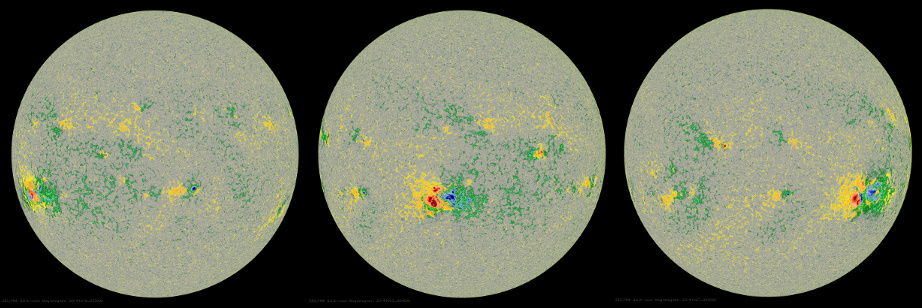
\includegraphics[width=14cm]{figs/2014_oct_sunspots.jpg}
\caption{SDO HMI colorized magnetogram images of solar active region AR 12192, taken
	on 10/19/2014, 10/23/2014, and 10/27/2014, respectively.  Simulated
	observables could mimic the behavior of regions such as this and help
	us understand when and why they release solar flares such as the X3.1
	flare released on 10/24/2014.
	\label{AR12192}}
\end{figure}

\section{Timeline of proposed work}
\paragraph{Year 1:}
Acquire access to ASH code and learn how to interface with it.
Create and execute first suite of simulations, successfully gathering
all data necessary to determine the role of the solar tachocline.  
Begin work on analysis routines.  
\vspace{-0.5cm}
\paragraph{Year 2:}
Analyze simulated data to gain an understanding of the tachocline's role in
generating the solar dynamo.  Publish a peer-reviewed article on the findings
of the simulations.  Research necessary techniques for and begin work on 
a second suite of simulations to be
used in the creation of simulated observables.  
\vspace{-0.5cm}
\paragraph{Year 3:}
Run second simulation set and create simulated observables, including data
directly comparable to that currently gathered by SDO and to be gathered by the
Solar Orbiter.  Compare the evolution of interesting simulated
events to similar observed events.  Make predictions on expected phenomena in
upcoming polar data from the Solar Orbiter.


\newpage

\section{Relevance to NASA} 
The proposed work fits with NASA's 2014 Strategic Plan objective
1.4:
``Understand the Sun and its interactions with Earth and the solar
system, including space weather.''
This work also fits in with one of the three overarching science goals
of the Heliophysics section of NASA's 2014 Science plan: 
``Develop the
knowledge and capability to detect and predict extreme conditions in space to
protect life and society and to safeguard human and robotic explorers beyond
earth.''  Furthermore, simulated observables created by this work will be
directly comparable to data retrieved by the currently operational Solar
Dynamics Observatory and the future NASA-ESA Solar Orbiter mission.

\section{Summary}
In order to predict extreme space conditions caused by the Sun's magnetic
activity, we must have an intricate understanding of the behavior of the Sun's
magnetic dynamo.  While solar dynamo theory has progressed impressively in
recent years, its progression has been marked by
a series of impressive simulations with no tangible connection to
observables that utilize an untested assumption as a theoretical cornerstone.
After recent simulations' disagreements regarding the 
tachocline's role in producing the solar magnetic dynamo, it is time
to put the assumed importance of the tachocline to the test.  Furthermore,
in order to have a
consistent, predictive theory on solar magnetism, it
is necessary to connect theoretical numerical simulations with tangible 
observables.  Only when these two sources of insight are brought together
will NASA's Science Plan goal of predicting extreme conditions in space
be realizable.  The wealth of Solar Dynamics
Observatory data available alongside the upcoming launch of the Solar Orbiter
set the present as the perfect time to connect theory and observation. 


\bibliographystyle{apj}
\begingroup
\renewcommand{\section}[2]{}%
\begin{footnotesize}
\bibliography{biblio}
\end{footnotesize}
\endgroup
\end{document}
